\label{cha:cobordisms}

We now delve into some arguments for smooth manifolds.
Once the general idea is in place, the following chapters make explicit the corresponding construction for triangulations of manifolds.

The problems of this chapter lie in the realm of cobordism.
\begin{defn}
  \label{def:cobordism}
  Let $W$ be a manifold with boundary $\pd W=M_1\cup M_2$.
  We say that $M_1$ and $M_2$ are \emph{cobordant} and $W$ is a \emph{cobordism} of the pair $(M_1,M_2)$.
\end{defn}
As discussed in the introduction, there are many ways to prove that a closed, oriented 3--manifold is cobordant to $\emptyset$.
Our goal is to take a 3--manifold triangulation $M$ and produce an explicit triangulated cobordism $W$ of the pair $(M,\emptyset)$.

\section{Morse Theory}
\label{sec:morsetheory}

Our primary use of Morse theory is to define a pair of related constructions.
The first is the \emph{handle decomposition} of a manifold, which comes with a dual decomposition.
The second is the \emph{Stein complex} of a Morse function on a manifold.
The main results from this chapter connect a Stein complex with a handle decomposition, and this construction is extended to triangulations in the remaining chapters.

\begin{defn}
  A generic smooth function $f:M\to\R$ where $M$ is an $n$--manifold is called a \emph{Morse function}.
  For a critical point $p\in M$ of $f$, the \emph{index} of $p$ is the dimension of the largest subspace of $T_p M$ such that $d^2f_p$ is negative definite.
  Less formally, this corresponds to the number of independent directions in $M$ along which $f$ decreases.
  We denote by $M^a$ the subspace $f\inv(-\infty,a\,]$ where $f$ is a fixed Morse function on $M$.
\end{defn}

A key question of Morse theory regards how the topology of $M^a$ changes as $a$ passes the critical values of $f$.
This question is answered by the following two theorems.

\begin{theorem}
  \label{thm:morseretract}
  Let $f:M\to\R$ be a Morse function with no critical values in $(a,b\,]$, $a<b$.
  If $f\inv[\,a,b\,]$ is compact, then $M^a$ and $M^b$ are diffeomorphic, and $M^b$ deformation retracts onto $M^a$.
\end{theorem}

\begin{theorem}
  \label{thm:morsehandle}
  Let $f:M\to\R$ be a Morse function.
  Let $p$ be a critical point of $f$ of index $\lambda$ with associated critical value $f(p)=q$.
  If $f\inv[\,q-\varepsilon, q+\varepsilon\,]$ is compact and contains no critical points other than $p$, then $M^{q+\varepsilon}$ is diffeomorphic to $M^{q-\varepsilon}\cup_\varphi H^\lambda$ for some attaching map $\varphi:S^{\lambda-1}\times\D^\mu\to \pd(M^{q-\varepsilon})$.
\end{theorem}

\begin{defn}
  Let $f:M\to\R$ be a Morse function on a closed $n$--manifold $M$ with critical points $\{p_1,\dots,p_k\}$ of indices $\{\lambda_1,\dots,\lambda_k\}$ and a set $\{t_0,\dots,t_k\}$ of numbers in $\R$ such that
  \[
	0\leq t_0 < f(p_1) < t_1 < f(p_2) < \cdots < t_{k-1} < f(p_k) < t_k \leq 1,
  \]
  and
  \[
	  \lambda_1 \geq \lambda_2 \geq \cdots \geq \lambda_k.
  \]
  The previous theorems guarantee that, for each $i\geq 1$, $f\inv[\,t_{i-1},t_i\,]$ is diffeomorphic to $(f\inv(t_{i-1})\times\I)\cup H^{\lambda_i}$, giving us a realization of $M$ as
  \[
	  \emptyset = M_0 \subset M_1 \subset M_2 \subset \cdots \subset M_{k-1} \subset M_k = M
  \]
  where $M_i$ is obtained from $M_{i-1}$ by attaching a $\lambda_i$--handle.
  Such a realization is called a \emph{handle decomposition} of $M$.
\end{defn}

A Morse function $f$ satisfying the requirements to define a handle decomposition actually defines two handle decompositions --- one from $f$ and one from $1-f$.
The handle decompositions from $f$ and $1-f$ are dual in the sense that every $\lambda$--handle attached in the making of the decomposition from $f$ has a corresponding $\mu$--handle in the decomposition from $1-f$.
This handle is realized by reversing the roles of the core and co--core in a given $\lambda$--handle $H^\lambda$ to obtain a $\mu$--handle $H^\mu$.

Similar results can be found for manifolds with boundary.
Let $W$ be an $n$--manifold with boundary $\pd W = M_0\sqcup M_1$, where both $M_0$ and $M_1$ are compact.
The Morse functions on $W$ that extend Theorems \ref{thm:morseretract} and \ref{thm:morsehandle} are those that fix $f(M_0)=0$, $f(M_1)=1$.
Now, the handle decomposition of $W$ is built on top of the component $M_1\times\{1\}$ of $M_0\times\I$, with $M_0\times\{0\}$ corresponding to the boundary component $M_0$ in the finished product.

\begin{defn}
  \label{def:morse2function}
  A generic smooth function $f:M\to\RR$ where $M$ is an $n$--manifold is called a \emph{Morse 2--function}.
\end{defn}

\begin{defn}
  \label{def:steinfactorization}
\end{defn}

\begin{defn}
  \label{def:steincomplex}
\end{defn}


\section{2--Manifolds Bound 3--Manifolds}
\label{sec:2bound3}

We now have the necessary framework to demonstrate that a closed, oriented 2--manifold bounds a 3--manifold through an explicit construction.
This is useful as a jumping off point for the case one dimension higher, that of 3--manifolds bounding 4--manifolds, which draws on the same framework and methods.

\begin{theorem}
	\label{thm:2bound3}
	Let $\Sigma$ be a closed orientable surface and $f:\Sigma\to[\,0,1\,]$ a proper Morse function with distinct critical values.
	Then there exists a cobordism of the pair $(\Sigma,\emptyset)$ with an explicit handle decomposition described fully by a Stein complex of $f$.
\end{theorem}

\begin{figure}
	\caption{A typical Morse function $T^2\# T^2\to\R$, its Stein factorization, and corresponding dual handle decomposition.}
	\centering
	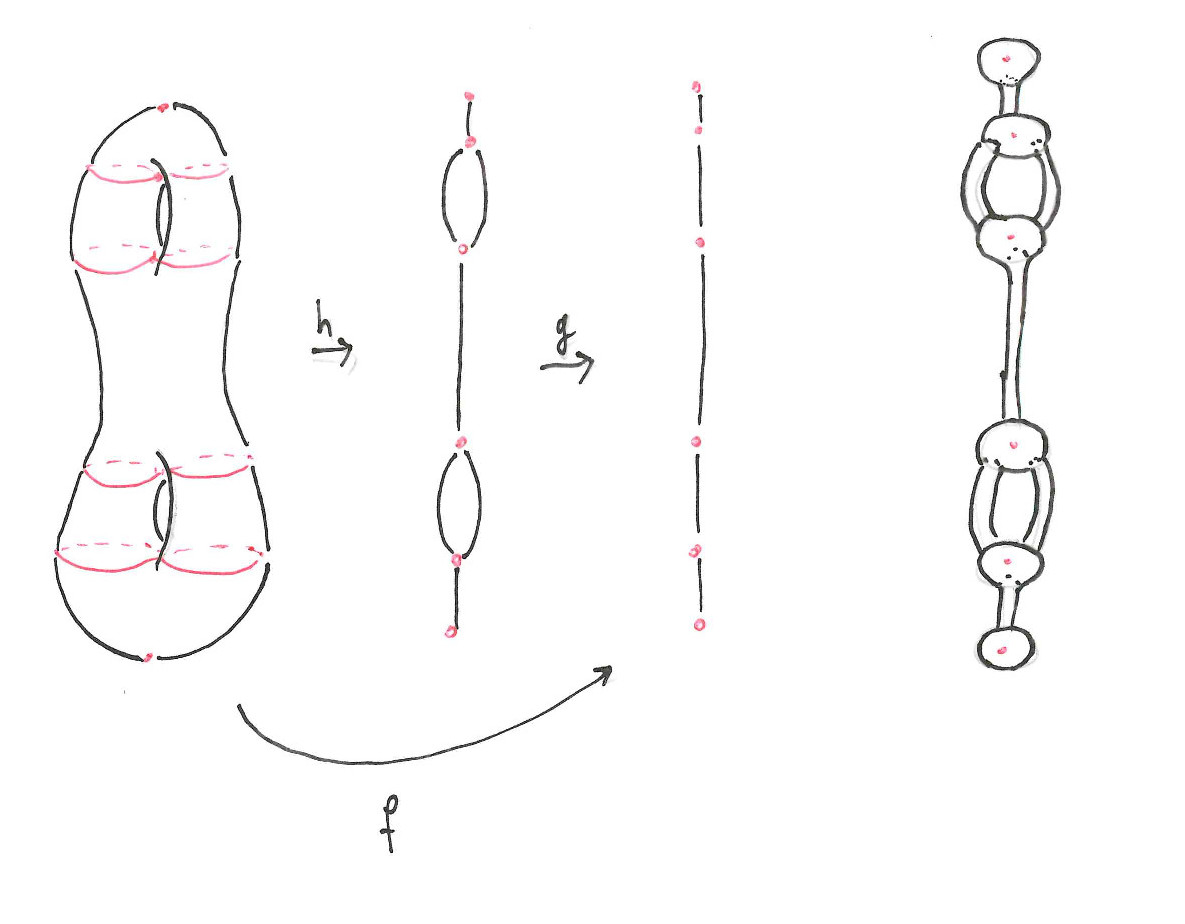
\includegraphics[height=4in]{figures/typicalmorse.jpg}
	\label{fig:typicalmorse}
\end{figure}

\begin{proof}
	Figure \ref{fig:typicalmorse} depicts a typical Morse function acting on the closed oriented surface of genus 2, and samples some of the notation we will define initially.
	We begin by examining the preimages of points $x\in\R$.
	Denote the space $f\inv(x)$ by $\Sigma_x$, a small interval around $x$ by $\varepsilon(x)=(x-\varepsilon,x+\varepsilon)$, and the neighbourhood in $\Sigma$ around $\Sigma_x$ by $f\inv(\varepsilon(x))=\varepsilon(\Sigma_x)$.
	The spaces $\Sigma_x$ and $\varepsilon(\Sigma_x)$ may not be connected, so we index the connected components by superscript.
	Let $p$ be a critical point of $f$ with critical value $f(p)=x$.
	By our assumption that critical values are distinct, $p$ is the only critical point of $f$ in $\Sigma_x$.
	The connected component of $\Sigma_x$ containing $p$ is called the \emph{singular fiber} at $p$ and is denoted $\Sigma_x^p$.
	The connected component of $\varepsilon(\Sigma_x)$ containing $p$ is called the \emph{critical neighbourhood} at $p$ and is denoted $\varepsilon^p(\Sigma_x)$.
	By the regular value theorem, any regular value pulls back through $f\inv$ to a disjoint collection of circles in $\Sigma$ called \emph{regular fibers}.
	Likewise, a neighbourhood $\varepsilon(x)$ that contains no critical values of $f$ pulls back to a disjoint collection of annuli in $\Sigma$.
	The restriction of $f$ to the components of $\Sigma_x$ that do not contain a critical point has $x$ as a regular value, so the remaining connected components of $\Sigma_x$ are all copies of $S^1$ that we index by $\Sigma_x^i$ for $i=1,\dots,k$, and their associated neighbourhoods are the annuli $\varepsilon^i(\Sigma_x)$.
	When referring to an arbitrary connected subspace of $\Sigma_x$ that could be the singular fiber $\Sigma_x^p$ or a regular fiber $\Sigma_x^i$, we will use the notation $\Sigma_x^*$.
	
	The shape of a singular fiber $\Sigma_x^p$ is determined by the index of $p$.
	Because $f$ is a Morse function whose domain is a surface, its critical points are easily classified by the Morse lemma (Lemma \ref{lem:morselemma}).
	Locally in $\Sigma$, a critical point of index 0 is a minimum, of index 1 a saddle, and of index 2 a maximum of $f$.
	
	Let $x$ be a critical value for the critical point $p$ and take $\varepsilon$ to be small enough that $\varepsilon(x)$ contains no critical values other than $x$.
	When $p$ is of index 0 or 2, we can immediately deduce that $\varepsilon^p(\Sigma_x)$ is diffeomorphic to a disc.
	When $p$ is of index 1, the Morse lemma tells us that $\Sigma$ looks like a standard saddle near $p$.
	The intersection of $\Sigma_x^p$ with this saddle is a cross whose centre is $p$.
	For $y\in\varepsilon(x)$, $y$ is a regular value whose preimage is a disjoint union of circles.
	The circles above and below the saddle singularity are the result of smoothing out the cross into a pair of oriented arcs, done in two possible ways.
	The orientations of these circles orient the cross, which has two incoming arms and two outgoing arms which appear in alternating order.
	A Morse function has distinct singular fibers, so the cross we know about in $\Sigma_x^p$ must have its arms connected in $\Sigma_x^p$ through nonsingular orientation--preserving arcs.
	We can then see that $\Sigma_x^p$ is a figure 8, and $\varepsilon^p(\Sigma_x)$ is a pair of pants in $\Sigma$.
	

	\begin{figure}
		\centering
		\caption{Smoothing a cross into a saddle}
		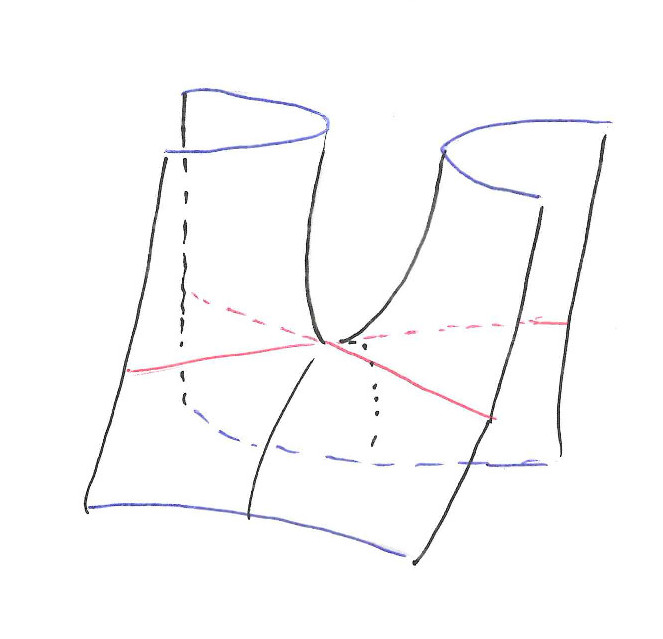
\includegraphics[height=3in]{figures/smoothcross.jpg}
		\label{fig:smoothcross}
	\end{figure}
	
	This analysis is sufficient to form a handle decomposition for a cobordism of $(\Sigma,\emptyset)$.
	We begin with the 3--manifold $\Sigma\times\I$ with boundary components $\Sigma_0=\Sigma\times\{0\}$ and $\Sigma_1=\Sigma\times\{1\}$, and let $f:\Sigma_0\to\I$ be a Morse function with distinct critical values $x_i$.
	The general idea is that we attach handles to $\Sigma_0$, altering that boundary component until it is empty.
	The $x_i$ partition $\I$ into open intervals containing only regular values.
	We take the associated regular annuli to be attaching regions for 3--dimensional 2--handles, and then fill in what remains with 3--dimensional 3--handles.
	
	For an interval $(x_i,x_{i+1})$, consider the subinterval $\varepsilon(t_i)$ where $x_i<t_i<x_{i+1}$ and $\varepsilon$ is small enough that $\varepsilon(t_i)$ contains neither $x_i$ nor $x_{i+1}$.
	Take the associated regular annuli $\varepsilon(\Sigma_{t_i})$ to be the attaching regions for 3--dimensional 2--handles.
	The boundary component that was once $\Sigma_0$ is now the result of removing the interiors of the annuli $\varepsilon(\Sigma_{t_i})$ from $\Sigma_0$ for each $t_i$, and then introducting discs parallel to the cores of the attached 2--handles.
	These discs are seen as $\DD\times\{0\}$ and $\DD\times\{1\}$ inside of a 2--handle $\DD\times\D^1$.
	The boundary circles of the discs are $\Sigma_{t_i-\varepsilon}$ and $\Sigma_{t_i+\varepsilon}$ for each $i$.
	
	There are now intervals about each critical point that we know, from our analysis above, pull back to discs, annuli, and pairs of pants.
	Each of these subsurfaces have circle boundaries that correspond to the regular fibers $\Sigma_{t_i-\varepsilon}$ and $\Sigma_{t_i+\varepsilon}$ which were capped with discs in the previous step.
	The altered boundary described before is therefore a collection of copies of $S^2$, which we take to be the attaching regions of 3--dimensional 3--handles.
	
	With these handles attached, we obtain $(\Sigma\times\I)\cup\{\textrm{2--handles}\}\cup\{\textrm{3--handles}\}$, which is a 3--manifold with exactly one boundary component of $\Sigma_1$, i.e. a cobordism of the pair $(\Sigma,\emptyset)$.
	
	The corresponding dual handle decomposition is realized by turning the process upside down.
	Where we previously had 3--handle attachments with cores $\D^3\times\{\vec{0}\}$ and cocores $\{\vec{0}\}\times\{\vec{0}\}$, we now have 0--handles with cores $\{\vec{0}\}\times\{\vec{0}\}$ and cocores $\D^3\times\{\vec{0}\}$.
	In other words, the dual construction begins by taking the disjoint union of a collection of 3--discs that correspond to the space obtained by capping the boundary circles of the components $\varepsilon(\Sigma_{x_i})$ with 2--discs and then filling the spheres with 3--balls.
	Where we previously had 2--handle attachments with cores $\DD\times\{\vec{0}\}$ and cocores $\{\vec{0}\}\times\D^1$, we now have 1--handle attachments with cores $\{\vec{0}\}\times\D^1$ and cocores $\DD\times\{\vec{0}\}$.
	In other words, we connect the 0--handles together using 1--handles.
	The old belt 0--spheres of the 2--handles in the previous construction correspond here to new attaching 0--spheres, and the attaching maps are chosen to preserve orientability cf.\ Remark~\ref{rmk:1handle}.
	The new attaching 0--spheres bound the new cores, the old core 2--discs are now cocores.
	This construction yields a 3--manifold whose boundary is exactly $\Sigma$, and is indeed another cobordism of the pair $(\Sigma,\emptyset)$.
	
	A Stein factorization $f=g\comp h$ is simple to describe.
	Define the equivalence relation $\sim$ on the points in $\Sigma$ by putting $p\sim q$ if and only if $f(p)=f(q)=x$ and $p$ and $q$ are in the same subspace $\Sigma_x^*$.
	Then $h$ is the quotient map $\Sigma\to \Sigma/\!\!\sim$ where the points of $\Sigma/\!\!\sim$ are the subspaces $\Sigma_x^*$, and $g$ is the map $\Sigma/\!\!\sim\, \to\R$ defined by $g(\Sigma_x^*)=x$.

	The Stein complex $S=\Sigma/\!\!\sim$ can be viewed as a graph $G$.
	A critical value $x=f(p)$ has an associated singular fiber $\Sigma_x^p$ in $S$, and possibly some copies of $S^1$ given by $\Sigma_x^i$.
	We take the associated points $h(\Sigma_x)$ in $S$ for each critical value to be the vertex set $v(G)$.
	For a pair of adjacent critical values $x_{j}$, $x_{j+1}$, an appropriate choice of $\varepsilon$ and $x\in(x_{j},x_{j+1})$ yields a collection of regular annuli $\varepsilon(\Sigma_x)$ in $\Sigma$ that has boundary inside of $\Sigma_{x_{j}}\cup\Sigma_{x_{j+1}}$.
	In $S$, we find $h(\varepsilon(\Sigma_x))$ to consist of 1--dimensional strands that connect components of $\Sigma_{x_{j}}$ and $\Sigma_{x_{j+1}}$.
	The set of pairs $(v,w)$ of connected subspaces with $v\in\Sigma_{x_{j}}$ and $w\in\Sigma_{x_{j+1}}$ such that $v$ and $w$ are connected by a strand in $S$ forms the edge set $e(G)$.
	
	At this point, $G$ corresponds exactly to the dual handle decomposition given earlier.
	For each vertex of $G$ we get a 0--handle.
	For each edge, a 1--handle.
	We attach 1--handles with only one demand: that the resulting space continues to be orientable.
\end{proof}

The Stein complex obtained in the proof of Theorem~\ref{thm:2bound3} may have superfluous vertices.
In particular, a vertex $v$ of $G$ that is adjacent to exactly two verticex $u$ and $w$ via the edges $(u,v)$ and $(v,w)$ may be replaced, along with its adjacent edges, by a single edge $(u,w)$.
To see that the handle decomposition described by this Stein complex graph is equivalent, examine the attaching region of the 1--handle corresponding to $(u,v)$ as it sits inside the boundary of the 0--handle corresponding to $v$.
This region may be isotoped over the 1--handle corresponding to $(v,w)$, where it ends up in the boundary of the 0--handle corresponding to $w$.
We are left with a 0--handle $v$ and 1--handle $(v,w)$ that are contractible into $w$.

\section{3--Manifolds Bound 4--Manifolds}
\label{sec:3bound4}

To extend the results of the previous section to the case of 3--manifolds bounding 4--manifolds, we consider generic proper smooth maps from closed orientable 3--manifolds into the 2--ball $B^2$.
Such a map is Morse--like in the sense that its singular set is well behaved, it can be studied via the same techniques as in Section \ref{sec:2bound3}, and we may recover a Stein factorization and Stein complex that define a handle decomposition for a bounding 4--manifold.

\begin{theorem}
	\label{thm:3bound4}
	Let $M$ be a closed orientable 3--manifold.
	Then a proper generic smooth map $f:M\to \BB$ determines a handle decomposition for a cobordism of the pair $(M,\emptyset)$.
\end{theorem}

\begin{proof}
	By Sard's theorem, the image of the singular set $f(s_f)$ in $\BB$ has Lebesgue measure 0.
	By genericity, and because the maps constructed in Chapter \ref{cha:alg1} satisfy this requirement, we take $s_f$ to consist of a set of arcs in the plane that intersect each other only pairwise and transversally, in such a way that $\BB\setminus s_f$ consists of a collection of regions $R_i$ homeomorphic to copies of $\BB$ along with a single annular region $R_\infty$ that does not intersect $f(M)$, and in such a way that $f(s_f)$ has a natural structure as a simple undirected 4--valent planar graph.
	We classify the critical values of $f$ as codimension 1 inside of arcs away from crossings, and codimension 2 at arc crossings.
	This classification makes the simple undirected planar graph structure of $f(s_f)$ explicit.
	The vertex set is given by the set of codimension 2 critical values and the edge set is the collection of codimension 1 critical values.
	
	We obtain a 4--manifold with boundary $M$ by attaching 2--handles corresponding to the regular regions $R_i$, 3--handles corresponding to codimension 1 singularities, and 4--handles corresponding to codimension 2 singularities.
	
	We will first focus on a region $R$ in $\BB$ that is not $R_\infty$.
	Begin by ``shrinking'' $R$ away from $f(s_f)$ into a space $\D$ that is homeomorphic to $\DD$
	Every point of $\D$ has preimage a disjoint collection of circles by the regular value theorem, so we centre our analysis on an arbitrary regular value $x$ and its regular fibers, where $M_{x,k}$ denotes the $k\nth$ regular fiber mapped over $x$ by $f$.
	An appropriate closed tubular neighbourhood of $M_{x,k}$ will consist entirely of regular fibers that map into $\D$ and has the structure of a closed 2--disc bundle over the circle, hence is a solid torus.
	The neighbourhood can be extended to enclose the entirety of $f\inv(\D)$.
	
	In summary, an arbitrary point $x_i$ is chosen from a closed 2--disc $D_i$ which itself is taken as a shrinking of an open region $R_i$.
	For each $k$, the $k\nth$ regular fiber $M_{i,k}$ over $x_i$ is taken as the zero section of a 2--disc bundle that maps over $D_i$.
	Such a bundle is an open solid torus, and the $k\nth$ bundle is denoted $V_{i,k}$.
	Of particular importance in $V_{i,k}$ are the zero section and a certain isotopy class of longitudes.
	The zero section $z(V_{i,k})$ is a regular fiber that maps over a point interior to $\D_i$, and the longitudinal isotopy class is the one that contains regular fibers that map to single boundary points of $D_i$.
	This pair determines an attaching map for 4--dimensional 2--handle attached over $V_{i,k}$.
	
	\begin{figure}
		\centering
		\captionsetup{justification=centering}
		\caption{Closed sleeve around an arc of codimension 1 critical values and the two neighbouring codimension 2 critical values}
		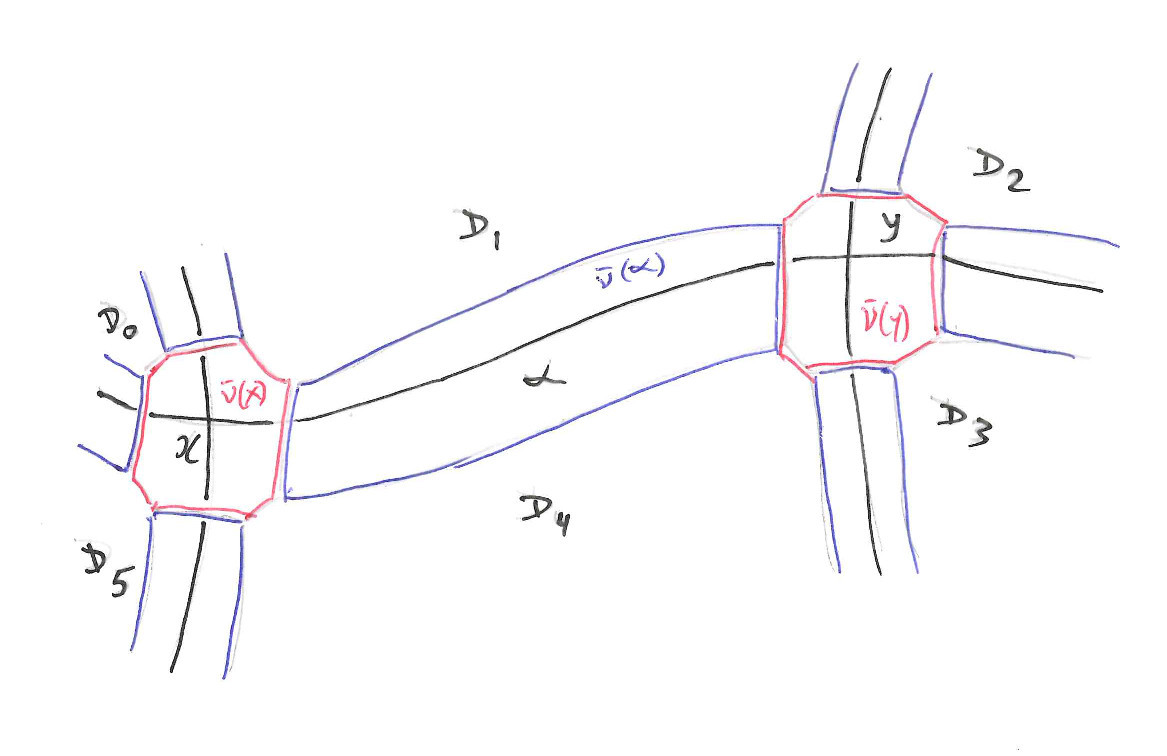
\includegraphics[height=4in]{figures/critsleeve.jpg}
		\label{fig:critsleeve}
	\end{figure}
	
	Consider an arc $\alpha$ of codimension 1 critical values that separates a pair of regions $R_i$ and $R_j$ where either $i$ or $j$ may be $\infty$.
	As when we considered regions, $\alpha$ has been shrunk away from the codimension 2 critical values it connects.
	Let $\nbhd{\alpha}$ be a closed ``sleeve'' around $\alpha$ whose boundary intersects the boundaries of $D_i$ and $D_j$ as in Figure \ref{fig:critsleeve}.
	The restriction of $f$ to the preimage of a linear transversal to $\alpha$ that connects $D_i$ and $D_j$ is, itself, a Morse function.
	The intersection with $\alpha$ is a critical point of this restriction, and the same techniques from the proof of Theorem \ref{thm:2bound3} may be applied to $f\inv(\nbhd{\alpha})$.
	A strand of singular fibers over $\alpha$ consists of an interval in the case of an extremum for the associated Morse function or an interval crossed with the figure 8 when the associated Morse function yields a saddle singularity.
	The critical neighbourhood $f\inv(\nbhd{\alpha})$ contains a connected component that is either $\DD\times\I$ when we have cross sectional extremum, or $P\times\I$, where $P$ is the pair of pants surface, i.e.\ the 2--sphere with three interior 2--balls removed, when the cross section yields a saddle.
	All remaining connected components are intervals crossed with regular annuli.
	We use $A=S^1\times\D^1$, alternatively the 2--sphere with two interior 2--balls removed, to denote an annulus, and find $A\times\I$ to be the form of all remaining connected components.
	
	Whenever one of the regions that $\alpha$ separates is $R_\infty$, the cross section necessarily gives us an extremum, and the critical neighbourhood over $\nbhd{\alpha}$ is $\DD\times\I$.
	We call $\alpha$ a \emph{definite fold} when the critical neighbourhood is $\DD\times\I$, and an \emph{indefinite fold} when the critical neighbourhood is $P\times\I$.
	
	Let $x$ be a codimension 2 critical value and $\nbhd{x}$ the closed neighbourhoods whose boundary agrees with the shrunken regions and arc sleeves it is near as in Figure \ref{fig:critsleeve}.
	The possible singular fibers over $x$ are cataloged in \cite{Saeki}, and Figure \ref{fig:saekising} displays them.
	The singular fibers over $x$ may be disconnected.
	When that is the case, the fibers have the form seen in our codimension 1 analysis.
	Otherwise, the singular fiber has the shape of a 4--valent directed graph.
	The regular fibers are still copies of $S^1$.
	In each case $f\inv(\nbhd{x})$ is a 3--dimensional thickening of the corresponding fibers, hence is a disjoint collection of handlebodies of genus 0,1,2, or 3.
	The neighbourhood of a regular fiber is still a solid torus, so all but at most two of the connected components of $f\inv(\nbhd{x})$ will be genus 1 handlebodies.
	
	\begin{figure}
		\centering
		\captionsetup{justification=centering}
		\caption{Possible singular fibers of a proper generic smooth map from an orientable 3--manifold to a surface}
		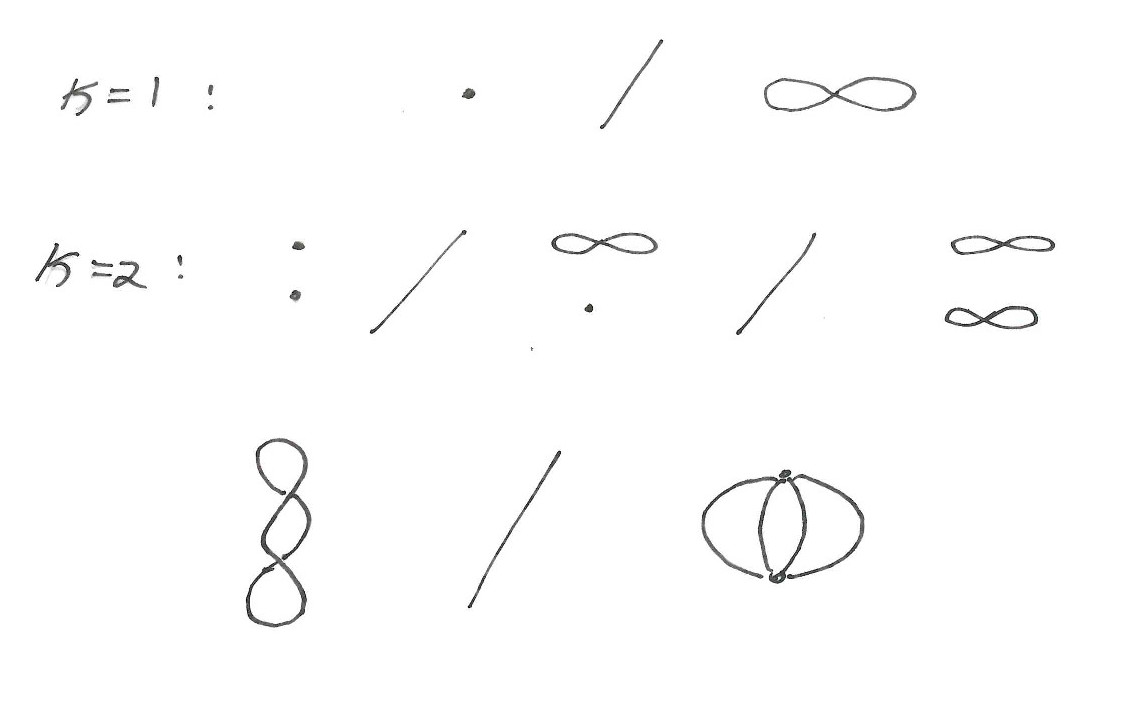
\includegraphics[height=3in]{figures/saekising.jpg}
		\label{fig:saekising}
	\end{figure}
	
	We may now begin describing a handle decomposition for a cobordism $W$ of the pair $(M,\emptyset)$.
	Begin with $M\times\I$, whose boundary is $M_0\sqcup M_1$ with $M_0=M\times\{0\}$ and $M_1 = M\times\{1\}$, and a proper generic smooth map $f:M_0\to\BB$.

	For each $i<\infty$ indexing the connected regions of $\BB\setminus f(s_f)$, we index over $k$ the connected components of $f\inv(R_i)$.
	Consider $D_i\subset R_i$, a 2--disc of regular values, and $V_{i,k}$, the $k\nth$ regular solid torus that maps over $D_i$.
	The solid torus $V_{i,k}$ has a trivial disc bundle structure over the regular fiber $M_{i,k}=z(V_{i,k})$, and $f(M_{i,k})=x$ in the interior of $\D_i$.
	Because we consider a single solid torus for the rest of this argument, we abbreviate $V_{i,k}$ to $V$, $M_{i,k}$ to $z(V)$ and $\D_i$ to $\D$.

	Let's remember what we're doing here --- we're attaching handles in such a way that, once all handles have been attached, the boundary component $M_0$ of $M\times\I$ has been filled in.
	In this step we attach 2--handles over $V$.
	Our goal is to do so in such a way that we remove the ``bad'' solid torus $V$ and replace it with a solid torus that is ``nice,'' where ``nice'' means that the newly introduced solid torus can be filled in by attaching 3-- and 4--handles.
	This happens by deleting $V$ and gluing 2--discs to the longitudes in $\pd V$ that are regular fibers of points in the boundary of $D$.
	To attach a 2--handle over $V$, we need
	\begin{enumerate}
		\item The isotopy class of an embedding $g:S^1\to M_0$, and
		\item the isotopy class of an identification $G:S^1\times\DD\to\nbhd{g(S^1)}$.
	\end{enumerate}
	The embedding $S^1\to M_0$ is easy enough to define as we will just be identifying $S^1$ with $z(V)$.
	This $S^1$ lives as the attaching sphere $S^1\times\{0\}$ inside of the 2--handle $\DD\times\DD$ that we plan to attach.
	Taking $\pd (\DD\times\DD)=(S^1\times\DD)\cup(\DD\times S^1)$ to be the genus 1 Heegard splitting of $S^3$, we will be defining a map $G:V\to S^1\times\DD$, where $S^1\times\DD$ is the first torus component.
	We call the other torus $V^*$.
	In order to satisfy our desired criteria, we need to have $G$ be in the isotopy class of a map that takes a regular fiber $J$ over a point in the boundary of $\D$ to $S^1\times\{1\}$.
	When this is true, we may form the adjunction $(M\times\I)\cup_{G\inv}(\DD\times\DD)$ and $J$ bounds a disc in $V^*$.
	Every fiber in the interior of $V$ now bounds a disc, and the new boundary is exactly $V^*$, whose meridians are the fibers that project over the boundary of $\D$.
	This is the property we wanted --- we've replaced the ``bad'' solid torus $V$ with the ``nice'' solid torus $V^*$.
	
	\begin{figure}
		\centering
		\captionsetup{justification=centering}
		\caption{The solid tori $V$ and $V^*$ with boundary curves $J$, $K$, and $L$.}
		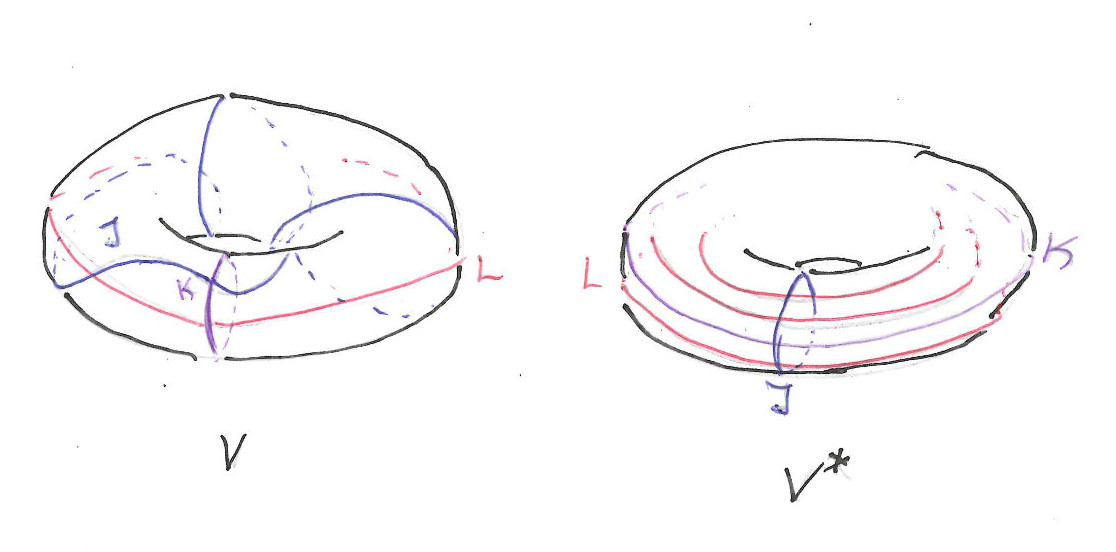
\includegraphics[width=6in]{figures/VV.jpg}
		\label{fig:VV*}
	\end{figure}
	
	A class $[G]$ satisfying the above is unique and it exists.
	To see why, let $\varphi:V\to S^1\times\DD$ be any trivialization of $V$, take $K=\varphi\inv(\{1\}\times S^1)$ to represent the meridinal isotopy class of $V$, and take $L$ be the longitude in $\pd V$ defined by $L=\varphi\inv(S^1\times\{1\})$.
	Let $J=f\inv(q)$ in $\pd V$ represent the isotopy class of regular fibers over boundary points of $\D$, where $q$ is an arbitrary point in the boundary of $D$.	
	Figure \ref{fig:VV*} shows the curves $J$, $K$, and $L$ with orientations sitting on $\varphi(V)$.
	Thinking of $S^1\times\DD$ as a subset of $\C^2$ gives it a natural orientation, which we have pulled back through $\varphi$ onto $K$ and $L$.
	We give $J$ a compatible orientation so that its intersections with $K$ and $L$ can be counted.
	Put $\kappa$ to be the oriented intersection number of $J$ and $L$.
	Then $\varphi(J)\in \pd\varphi(V)$ is in the isotopy class of $h_M^{\kappa}(\varphi(L))$, where $h_M$ is the meridinal twist defined in Theorem \ref{thm:mpgV}.
	Take $G=H_M^{-\kappa}\comp\varphi$, where $H_M$ is the extension of $h_M$ to the solid torus defined in Remark \ref{rmk:2handle}.
	In the boundary of $G(V)$, $G(J)$ is in the isotopy class of $S^1\times\{1\}$, $G(K)$ is in the isotopy class of $\{1\}\times S^1$, and $G(L)=h_M^\kappa(S^1\times\{1\})$.
	Existence of $G$ is shown, and uniqueness up to isotopy comes from the same uniqueness in trivializations of $V$ and of $H_M$.
		
	With 2--handles attached, we move onto the preimages of arc sleeves.
	Let $\nbhd{\alpha}$ be an arc sleeve, and consider the connected components of $f\inv(\nbhd{\alpha})$.
	Figure \ref{fig:arcsleevepre} displays the possible connected components of arc sleeve preimages, each of which has the form of a surface crossed with the interval.
	The boundary circles of these surfaces at a cross section $\Sigma\times\{t\}$ project through $f$ over the boundaries of shrunken regions, so they are filled with discs that sit inside of attached 2--handles from the previous step.
	In each case, we obtain a copy of $S^2\times\D^1$ over which we attach a 3--handle.
	The further modification to $M_0$ that takes place when we attach 3--handles can be thought of as the deletion of a copy of $S^2\times D^1$ followed by gluing 3--discs over the newly created 2--sphere boundary components.
	
	\begin{figure}
		\centering
		\captionsetup{justification=centering}
		\caption{Possible connected components of arc sleeve preimages}
		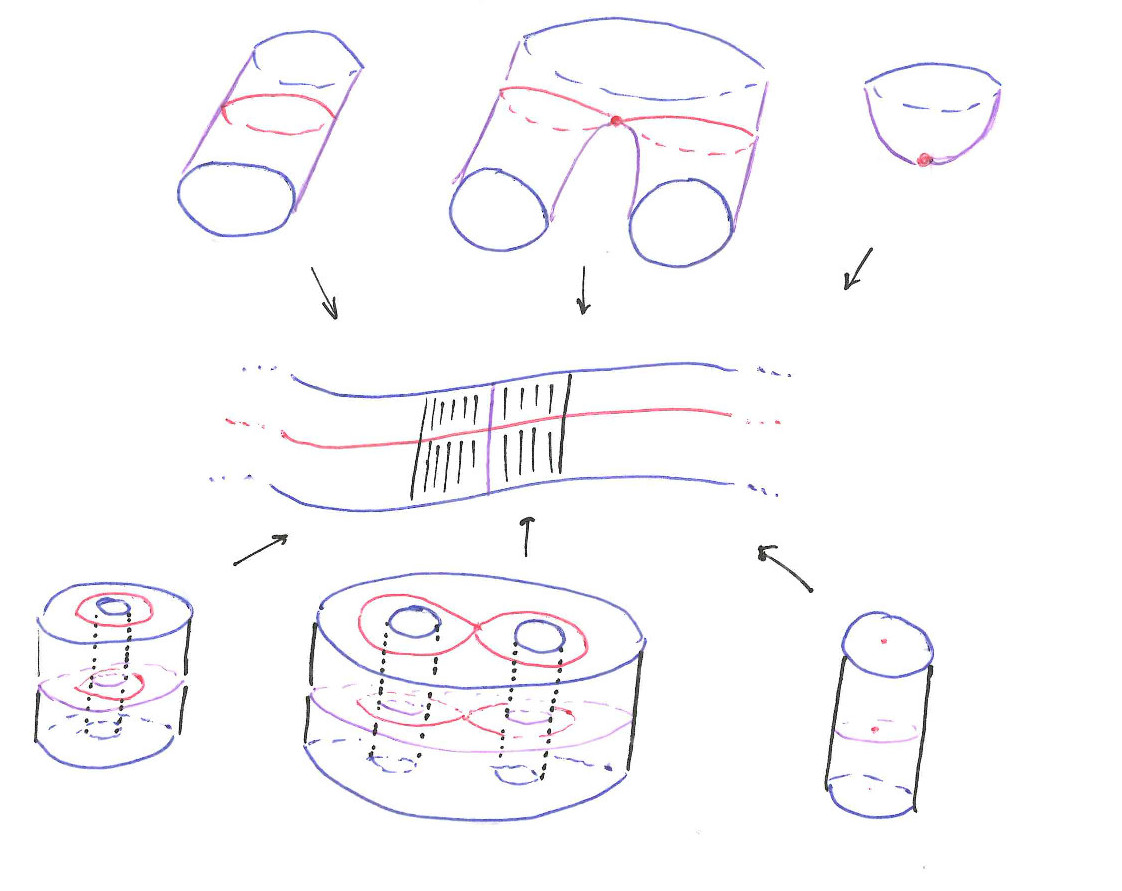
\includegraphics[height=4in]{figures/arcsleevepre.jpg}
		\label{fig:arcsleevepre}
	\end{figure}
	
	Finally, let $x$ be a codimension 2 critical value and let $\nbhd{x}$ be its sleeve.
	We find $x$ at the crossing of a pair of strands of codimension 1 critical values, and those strands are classified as definite or indefinite folds.
	The analysis of the codimension 2 critical value is then broken down into five cases.
	In four cases, we are able to extend the codimension 1 situation.
	This happens when the singular fiber is disconnected, called an \emph{uninteractive} singular fiber, or when one of crossing folds is definite.
	When both folds are indefinite and the singular fiber is connected, then the singular fiber is called \emph{interactive} and we defer to the analysis in \cite{CostThur08}.
	
	First we look at the connected components of $f\inv(\nbhd{x})$ that do not contain a singular fiber over $x$.
	These connected components are made from regular fibers, i.e.\ circles, that project over $\nbhd{x}$, i.e. a 2--disc.
	As in the case of regions of regular values, they are solid tori $V_{x,k}$, using the same naming convention that has been established for solid tori that map over the regions $D_i$.
	Seeing $V_{x,k}$ as a 2--disc bundle over $f\inv(x)$, we can find an isotopy class of longitudes that project over single points in the boundary $\pd\nbhd{x}$.
	These longitudes bound discs introduced during 2-- and 3--handle attachment.
	The union of all such discs yields a solid torus $V_{x,k}^*$ in the boundary.
	The boundary component consisting of $V_{x,k}$ and $V_{x,k}^*$ is described by the Heegaard splitting $V_{x,k}\cup_\varphi V_{x,k}^*$ where $\varphi$ takes a longitude of $V_{x,k}$ to a meridian of $V_{x,k}^*$.
	This is the standard genus 1 Heegaard splitting of $S^3$, so we have a copy of $S^3\times\D^0$ over which we may attach a 4--handle.

	The component that comes from an uninteractive definite fold is of the form $\DD\times\I$ as in the case of codimension 1 critical values.
	The 2--sphere boundary of this shape is filled with 2--discs from our 2-- and 3--handles, so this shape is the adjunction of a pair of 3--discs glued over their boundary.
	This is the genus 0 Heegaard splitting of $S^3$, so we have a copy of $S^3\times\D^0$ over which we may attach a 4--handle.
		
	\begin{figure}
		\centering
		\caption{Destabilizing pairs for the pair of pants}
		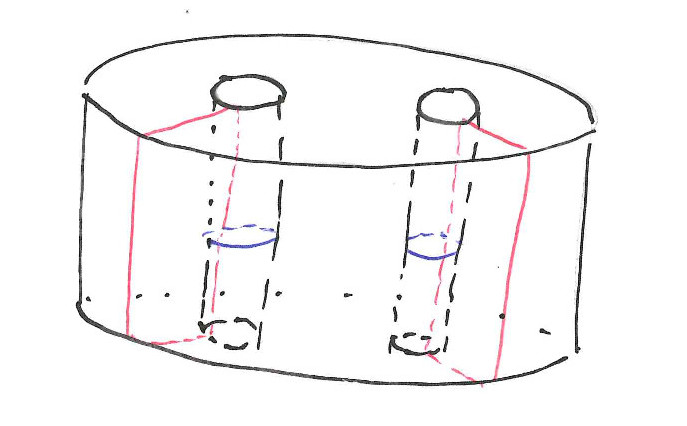
\includegraphics[height=3in]{figures/destabpants.jpg}
		\label{fig:destabpants}
	\end{figure}
		
	An uninteractive singular fiber that comes from an indefinite fold is the figure 8, and the preimage $f\inv(\nbhd{x})$ is a closed tubular neighbourhood of the figure 8 graph, which is homeomorphic to the pair of pants crossed with an interval.
	Here, we find a Heegaard splitting of genus 2 with two destabilizing pairs, showing that the splitting is a splitting of $S^3$, and we can attach a 4--handle to it by Theorem \ref{thm:lilwald}.
	An appropriate choice of meridians in $f\inv(\nbhd{x})$ would be a pair of curves that run from cuff to waist along the inside of each of the legs in the pair of pants, crest the waist, then down the outside of the legs back to the cuff.
	Meridians for the solid filled by our 2-- and 3--handles would run around the cuffs of each leg.
	Figure \ref{fig:destabpants} illustrates the idea.
	
	When an indefinite and definite fold interact, we get the same shapes found in the case of an uninteractive definite fold.
	From a 1--dimensional Morse function viewpoint, we witness a homotopy of a pair of peaks separated by a saddle come together into a single peak, eliminating the saddle.
		
	This leaves us with the case of interacting indefinite folds.
	The full analysis is covered in Section 4.4 of \cite{CostThur08}.
	They show that filling in $f\inv(\pd\,\nbhd{x})$ with 2--discs and gluing the two genus 3 handlebodies together over $f\inv(\pd\,\nbhd{x})$ results in a Heegard splitting of $S^3$ by explicitly finding 3 destabilizing pairs.
	We attach 4--handles over these 3--spheres.
	Attaching a 4--handle over a 3--sphere fills in the 3--sphere with a 4--disc, so these final modifications completely eliminate what is left of $M_0$.
	We are left with a handle decomposition for a cobordism of the pair $(M,\emptyset)$ built on top of $M_0$ in $M\times\I$.
\end{proof}

Let $f:M:\to\BB$ be a proper generic smooth function and $W$ a the cobordism of the pair $(M,\emptyset)$, both as per the construction in Theorem \ref{thm:3bound4}. 
Because the handle decomposition produced for $W$ consists of handles of index 2,3, and 4, the associated dual decomposition contains handles of degree 0,1, and 2.
Our goal is to obtain a combinatorial description of this decomposition, and we find this through the Stein complex.

Recall that the Stein complex for a Morse function on a surface was given by a 1--complex.
In the case of a proper generic smooth map $M\to\BB$, the Stein complex is given by a 2--complex $S$.
The vertices of $S$ correspond to 0--handles, the edges to 1--handles and the 2--cells to 2--handles.

We define the Stein factorization and complex of $f$ as usual.
Let $\sim$ be an equivalence relation on $M$ defined by $p\sim q$ if and only if $f(p)=f(q)=x$ and $p$, $q$ are in the same connected component of $f\inv(x)$.
Then $f=g\comp h$ where $h$ is the quotient map $M\to M/\!\!\sim$ and $g$ takes a point in $f\inv(x)$ to $x$.

\begin{theorem}
	\label{thm:stein2complex}
	Let $f$, $M$, $S$, and $W$ be as we defined above.
	Then $S$ is a 2--dimensional CW--complex that embeds flatly in $W$.
\end{theorem}

\begin{proof}
	There are only a few locations where $S$ could fail to be a CW--complex, and those are found over the critical values of $f$.
	We construct $S$ as we would any other CW--complex, by iteratively attaching cells of increasing dimension, and define a map $\varphi:S\into W$ that is almost a flat embedding in a similar fashion.
	Let $S$ be empty and begin by adding 0--cells to $S$.
	
	For a codimension 2 singular value $x$ of $f$, the fibers of over $x$ were discussed in Theorem \ref{thm:3bound4}.
	The Stein factorization $f=g\comp h$ has $h$ crush each fiber to a point, which we take as a new 0--cell in $S$.
	Let $\nbhd{x}$ be a sleeve of $x$ as in Theorem \ref{thm:3bound4}.
	In the construction of $W$, we attached 4--handles over 3--spheres with Heegaard decompositions over $f\inv(\nbhd{x})$.
	The cocore of a 4--handle is a single point, so we associate the 0--cells of $S$ with the cocores of 4--handles in $W$.
	Let $x_i$ be a fiber over $x$, let $H_i^4\subset W$ be the 4--handle associated to $x_i$, let $c_i\in H_i^4$ be the cocore of $H_i^4$, and let $v_i$ be the vertex of $S$ associated to $x_i$.
	Define $\varphi(v_i)=c_i$.
	
	We can now add edges to $S$.
	Let $\alpha$ be an open strand of codimension 1 critical points of $f$ with $\pd\overline\alpha=\{x,y\}$, a pair of codimension 2 critical points of $f$.
	Pulling back $\alpha$ to $M$ yields an open interval crossed with the fibers over any point of $\alpha$ and pulling back $\overline\alpha$ connects the fibers over $x$ and $y$.
	For a fiber $\alpha_i$ over $\alpha$ with endpoints $\alpha_i^x$ sitting inside of a fiber over $x$ and $\alpha_i^y$ sitting in a fiber over $y$, we add an edge attached over the vertices $v_i^x$ and $v_i^y$ associated to the fibers over $x$ and $y$.
	This corresponds to the action of $h$ on $\alpha_i$, which crushes the interval of fibers to an interval.
	
	Let $\nbhd{\alpha}$ be a sleeve of $\alpha$ as in Theorem \ref{thm:3bound4}.
	To construct $W$ we attached 3--handles over copies of $S^2\times\D^1$, those $S^2\times\D^1$ contained copies of $\Sigma\times\D^1$ with $\Sigma$ the 2--sphere with one, two, or three open 2--balls removed, and those $\Sigma\times\D^1$ projected over $\nbhd{\alpha}$.
	The cocore of a 3--handle is a copy of $\D^1$, which corresponds to an edge in $S$.
	Let $\alpha_i$ be a fiber over $\alpha$, $H_i^3$ the 3--handle associated with $\alpha_i$, $c_i$ the interval cocore of $H_i^3$, and $e_i$ the edge of $S$ corresponding to $\alpha_i$ with $\pd e_i=\{u,v\}$.
	Because $e_i$ is a 1--cell, it is homeomorphic to an interval $[\,0,1\,]$, so we take a slightly smaller closed subinterval $e_i'$ in $e_i$ (just as we can take $[\,\varepsilon,1-\varepsilon\,]$ inside of $[\,0,1\,]$) and define $\varphi(e_i')=c_i$.
	The endpoints of $c_i$ are the belt sphere of $H_i^3$, and they intersect the 4--handles $H_u^4$ and $H_v^4$ corresponding to $u$ and $v$.
	The intersection points are in the boundary 3--spheres of these 4--handles, so there are straight lines inside of the 4--handle that connect the cocore to these boundary points.
	Define $\varphi$ on $e_i\setminus e_i'$ to be those straight line segments in the appropriate continuous way.
	
	And finally, the 2--cells.
	Let $R$ be an open ball of regular values in the plane, and let $D$ be the 2--disc inside of $R$ that pulls back through $f$ to a disjoint collection of solid tori over which we attached 2--handles in our construction of $W$.
	Let $H$ be the 2--handle attached over a solid torus $V$ projecting over $D$.
	The boundary of $H^2$ is a 3--sphere with genus 1 Heegaard splitting consisting of $V$ and a dual torus $V^*$.
	We attached $H^2$ because we wanted to fill the boundary of $V$ with 2--discs that were easy to attach 4-- and 3--handles over, and $V^*$ is also contained in the union of these 4-- and 3--handles.
	The vertices and edges of $S$ corresponding to this collection 4-- and 3--handles forms a cycle $C$ in the 1---skeleton of the Stein complex already built.
	We know that $R$ contains only regular values, so it pulls back to a disjoint collection of open solid tori.
	Let $U$ be the open solid torus in this collection with $f(U)=R$ and $V\subset U$.
	In particular, $\pd V=\pd V^*\subset U$.
	The fibers of $S$ are fibers of $f$ that project over the regular values in $R$, so $h(U)$ is a 2--ball.
	The closure of $U$ intersects the singular fibers corresponding to the 4-- and 3--handles that contain $V^*$.
	We take $h(U)$ in $S$ to be a 2--cell attached over $C$.

	To define $\varphi$ on the 2--cell $\sigma_U$ corresponding to $U$, we start by defining it on $\sigma_V$, a subdisc of $\sigma_U$ (cf.\ the case of defining $\varphi$ on the edges of $S$, where $\sigma_V\subset\sigma_U$ just like how $\{z\in\C:|z|^2\leq 1-\varepsilon\}\subset\DD$).
	Recall that	$H^2$ is the 2--handle attached over $V$.
	It is useful to think of $H^2$ as a $\DD$ bundle over $\DD$, where the base space and zero section are the cocore $C_V$ of $H^2$.
	We define $\varphi(\sigma_V)=C_V$, and then examine the intersection of $C_V$ with the 4-- and 3--handles of $W$.
	The collection of higher index handles that intersect $H^2$ is exactly the collection that contains $V^*$, and the intersection is exactly $V^*$.
	The cocore $C_V$ intersects $V^*$ in exactly the belt sphere of $H^2$.
	We then extend $\varphi$ to $\sigma_U\setminus\sigma_V$ exactly as we did with the edges of $S$, by connecting the belt sphere of $H^2$ with the cocores of the 4-- and 3--handles by line segments.
	
	This demonstrates first that the Stein complex $S=h(M)$ has the structure of a 2--complex.
	Secondly, the map $\varphi:S\into W$ constructed here is piecewise--linear where it is not smooth, so can be smoothed into a flat embedding of a CW--complex.											
\end{proof}

In Section \ref{sec:proj} it is convenient to remove open balls from a given 3--manifold $M$ and build a projection of $M'$ instead.
We want the results of this section to still apply, so we state this in Theorem \ref{lem:stillworks}

\begin{lem}
	\label{lem:stillworks}
	Let $M$ be a closed orientable 3--manifold, and let $M'$ be $M$ with a finite number of disjoint 3--balls removed.
	Call the disjoint 2--sphere boundary components of $M'$ by $pd_i M'$.
	Let $f:M'\to\DD$ be a proper generic smooth map such that $f(\pd M')$ is a disjoint collection of intervals in the boundary of $\DD$ and the image of the singular set of $f$ away from $\pd M'$ is as described in the proof of Theorem \ref{thm:3bound4}.
	Then the Stein complex recovered for $f$ in the manner of Theorem \ref{thm:stein2complex} is exactly the Stein complex recovered for an extension of $f$ to $M$.
\end{lem}

\begin{proof}
	The singular fibres near $f(\pd M')$ are all definite folds, and extending $f$ to 3-balls attached over the boundary components of $M'$ yields an extension of that definite fold over the image of the 3--ball.
\end{proof}

All that's left is to realize the Stein complex as a set of instructions to build a handle decomposition of $W$, dual to the one obtained in Theorem \ref{thm:3bound4}, that relies only on $f$ and $S$.
We state this more precisely in Theorem \ref{thm:3stein4}.

\begin{theorem}
	\label{thm:3stein4}
	Let $f$, $M$, $S$, $W$ be as defined above.
	Then there exists a 4--manifold $W^*$ that is a cobordism of the pair $(M,\emptyset)$ in which $S$ embeds flatly as in Theorem \ref{thm:stein2complex}, and this manifold may be reconstructed from the combinatorics of $S$ and the map $f$.
\end{theorem}

\begin{proof}
	Let $G$ be the 1--skeleton of $S$.
	We consider first the 4--handlebody obtained by attaching to $\emptyset$ a 4--dimensional 0--handle $H_v^0$ for each vertex $v$ of $G$, embedding $v$ as the core of $H_v^0$, attaching a 1--handle $H_e^1$ with orientation preserving attaching maps into $\pd H_u^0$ and $\pd H_v^0$ for each edge $e=(u,v)$ of $G$, embedding $e$ as the core of $H_e^1$ plus a pair of line segments to the cores $\pd H_u^0$ and $\pd H_v^0$.
	The result is a 4--dimensional handlebody called the \emph{4--thickening} of $G$, and is denoted by $H_4(G)$.
	
	Consider now $U_S(G)$, a closed regular neighbourhood of $G$ in $S$.
	This is equivalent to $S$ minus an open ball inside of each 2--cell (as in Theorem \ref{thm:stein2complex} when we considered $\sigma_U\setminus\sigma_V$), or can also be seen as $G$ plus an annulus attached by one of its boundary components over each cycle that a 2--cell was attached over in Theorem \ref{thm:stein2complex}.
	In either case, $U_S(G)$ collapses onto $G$ and the 4--thickening of $U_S(G)$ is homeomorphic to the 4--thickening of $G$.
	To build $W$, we make a 3--thickening of $U_S(G)$, and then a 4--thickening of the 3--handlebody obtained.
	This time, however, we pay attention to how the 2--cells of $S$ interact with the thickening.
	
	We built $S$ to have a 1--skeleton $G$ whose interior vertices are all of degree 4 and whose boundary vertices are all of degree 3.
	The 3--thickened regular neighbourhoods of the five possible vertex types and the three possible edge types in $S$ are depicted in Figure \ref{fig:3thickeningblocks}.
	We use these to build the 3--thickening $H_3(U_S(G))$ of $U_S(G)$ where $U_S(G)$ is embedded in $H_3(U_S(G))$ and intersects the boundary of $H_3(U_S(G))$ in the curves depicted on the blocks in Figure \ref{fig:3thickeningblocks}.
	Thinking of $H_3(U_S(G))$ as generically a bundle of $\II$ over $U_S(G)$, the curves would be the zero section of the bundle over the boundary of $U_S(G)$.
	Once we have $H_3(U_S(G))$, there is a unique orientable $\II$ bundle over $H_3(U_S(G))$, and this is the 4--thickening of $G$.
	This bundle can be obtained either by specifying local trivializations that reverse the orientation of the $\II$ factor along the curves in $H_3(U_S(G))$ along which the space becomes nonorientable, or by first building the 3--thickening of $T\subset G$, a maximal spanning tree of $G$, 4--thickening that space, and then attaching all remaining 1--handles in the unique orientation preserving way.
	We choose the second construction.
	
	\begin{figure}
		\centering
		\captionsetup{justification=centering}
		\caption{3--thickening blocks for the 1--skeleton of the Stein complex}
		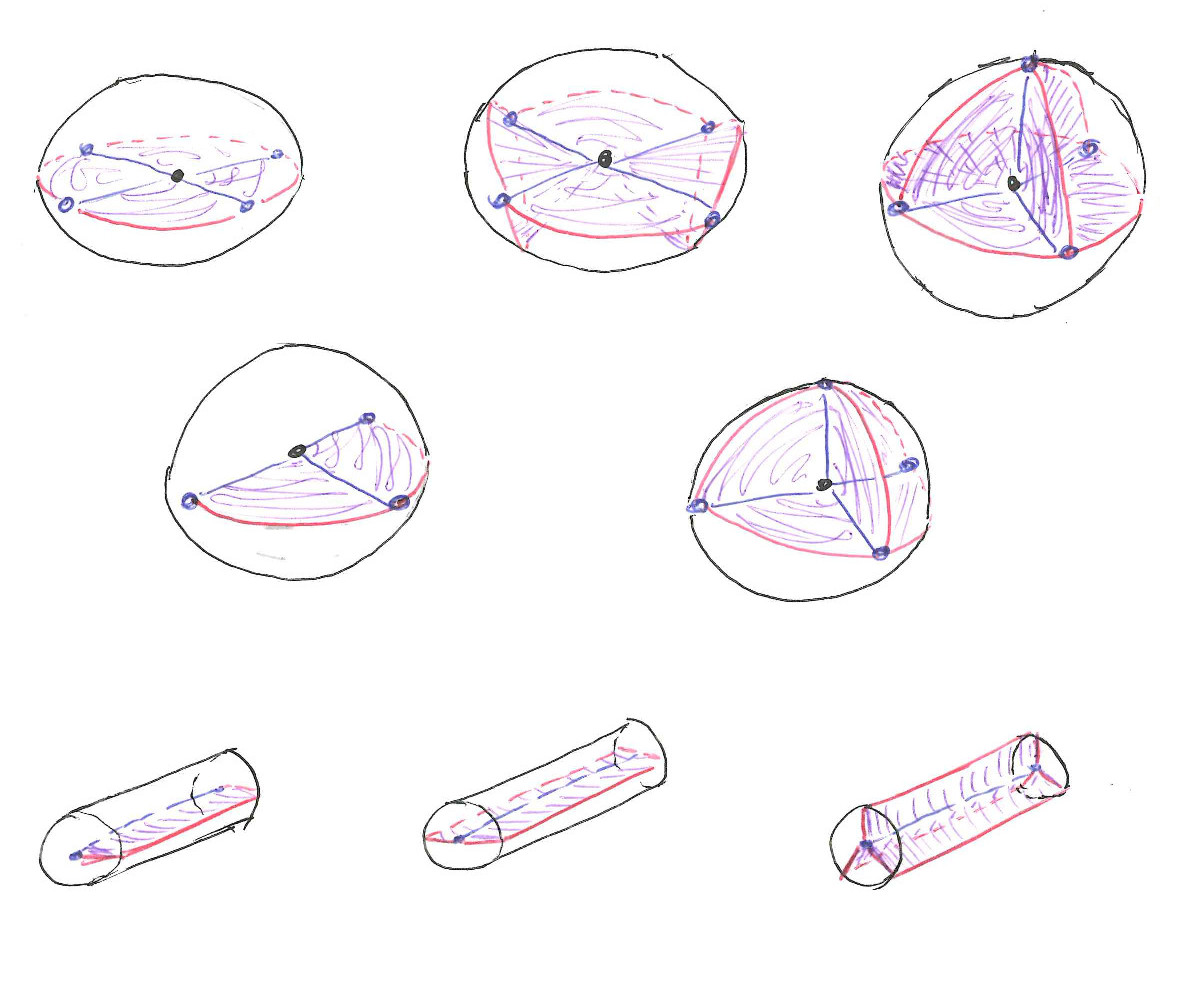
\includegraphics[width=6in]{figures/3thickeningblocks.jpg}
		\label{fig:3thickeningblocks}
	\end{figure}
	
	Building $H_3(U_S(T))$ by adding an appropriate vertex block to $H_3(U_S(T))$ for each vertex of $T$, then connect them together with edge blocks in the unique way that is forced by the combinatorics of $S$ for each edge of $T$.
	Take the product of this space with $\II$.
	The result is a $\II$--bundle over $H_3(U_S(T))$ and generically a $\II^2$--bundle over $U_S(T)$.
	To extend this to $G$, we add 1--handles for each edge in $G$ that is not in $T$.
	Every such edge has at least one 2-handle in $S$ attached over it, and every 2--cell of $S$ attaches over at least one edge added in this step.
	We use the product of our edge blocks with $\II$ as the 4--disc structure for our 1--handles.
	The combinatorics of $S$ and the requirement that $H_4(U_S(G))$ is orientable make these handle attachments unique.
	Our 4--thickening $H_4(U_S(G))$ is once again a $\II$--bundle over $H_3(U_S(G))$ and generically a $\II^2$--bundle over $U_S(G)$.
	The boundary circles of $U_S(G)$, corresponding to 2--cells of $S$ and thus 2--handles of $W$, are now thickened to solid tori in $H_4(U_S(G))$.
	The last step to this construction is the attachment of 2--handles over these solid tori. 
	
	Let $v^*$ be a boundary circle of $U_S(G)$ corresponding to a 2--cell $c_v$ of $S$ with thickening $V^*$ in the boundary of $H_4(U_S(G))$.
	The first thing we must do is specify a canonical 0--framing on $V^*$, which we do by investigating the diagonal of the square fibers $\II$.
	As a subspace of $V^*$, the union of the fibers have the structure of an annulus or a M\"obius strip.
	To see which we get, we turn to the completion of $H_4(U_S(T))$ into $H_4(U_S(G))$ accomplished by attaching 4--dimensional 1--handles.
	At least one such 1--handle corresponded to an edge of $\pd c_v$, and $n$ of them were attached with an orientation reversal in both $\II$ factors.
	If $n$ is even then the diagonal is an annulus and we put the canonical 0--framing as the trivialization that takes one boundary component of that annulus to $S^1\times\{1\}$.
	If $n$ is odd then the diagonal is a M\"obius strip.
	In this case we take a curve that follows one half of the boundary component of the M\"obius strip (i.e. once around $V^*$ in the longitudinal direction along the boundary), then connects to itself via one half positive twist in the orientation of $V^*$ (which is canonically oriented by the canonical orientations of the double intervals $\II$).
	
	With a 0--framing specified, we just need framing coefficients.
	To recover those, we ask how our canonical framing sits inside of $M$.
	This question is well defined because the solid tori we are attaching 2--handles over are the $V^*$ we examined in the proof of Theorem \ref{thm:3bound4}, and the boundaries of these tori are contained in $M$.
	
	The complex $S$ embeds flatly into $W$, and the restriction of that embedding to the 0-- and 1--handles of $W$ is exactly how $U_S(G)$ embeds in $H_4(U_S(G))$.
	Specifically, the zero section of the torus $V^*$ above is the belt sphere of the 2--handle in $W$ corresponding to the 2--cell $c_v$ in $S$.
	This belt sphere is then the attaching sphere of the dual 2--handle in the handle decomposition of $W^*$ and the framing coefficient is then the number of meridinal twists from the 0--framing to the longitude in $V^*$ that is a meridian of $V$.
	Attaching a 2--handles over every such $V^*$'s yields a handle decomposition of a 4--manifold $W^*$ that is dual to the decomposition of $W$ acquired in Theorem \ref{thm:3bound4}.
	We conclude that $W^*$ is the desired cobordism of $(M,\emptyset)$.
\end{proof}

There are a couple of points left to address in this chapter.
The first is that of explicitly recovering the 0--framing curve used in the attachment of 2--handles in Theorem \ref{thm:3stein4}, a necessity for turning this process into an algorithm.
The second is an acknowledgment of the origin of the ideas in this Section.

The 0--framing $L$ is a curve in the shared boundary of $V$ and $V^*$ that is a number of meridinal twists of $V^*$ away a meridian of $V$.
This number is the framing coefficient we equip to the 2--cell of $S$ representing 2--handle attachment over $V^*$ in the construction of $W^*$.

Because $L$ is a longitude of $V^*$, it wraps exactly once around the meridinal direction of $V$, and can thus be realized as a section over $\pd \D$ where $f(V)=\D$.
Let $\D_0$ be the zero section of $V$ as a disc bundle over an interior regular fiber of $V$.
Then the oriented intersection number of $J$ with $D$ yields the framing coefficient.
We compute the framing coefficient for a 2--cell of $S$ in Section \ref{sub:gleams} using this method.


This work is based on that of Costantino and Thurston in \cite{CostThur08} and of Turaev in \cite{Turaev91}.
Theorem \ref{thm:3stein4} in particular is a version of the Turaev Reconstruction Theorem.
Three distinct versions can be found as Theorem 4.1 of \cite{Cost05}, 3.8 of \cite{CostThur08}, and 19.1 of \cite{Turaev91}.
The proof presented is closest in form to that found in \cite{Cost05}.
These selections offer a decent introduction to the theory of shadows of 4--manifolds.
A shadow is a 2--complex with extra structure, and the Stein complex found in this section is almost a shadow.

%\section{Shadows of 3-- and 4--Manifolds}
%\label{sec:shadow}

The building instructions mentioned in the previous section were studied by Turaev in ~\cite{Turaev91} and are called \emph{shadows}.
Shadows are piecewise--linear 2--dimensional structures that live inside of piecewise--linear, compact, oriented 4--manifolds.
The central algorithm of this work uses shadows of 3-- and 4-- manifolds to construct a triangulation of a 4--manifold with a given 3--manifold boundary.

\begin{defn}
  Let $P$ to be a compact topological space.
  If every point $p$ of $P$ has a neighbourhood homeomorphic to an open set in one of the following local models
  \begin{enumerate}
    \item the closed 2--disc $D^2$,
    \item the product of the interval $I=[0,1]$ with the $Y$--shaped graph $K_{1,3}$, or
    \item the cone on the complete graph $K_4$,
  \end{enumerate}
  then $P$ is a \emph{simple polyhedron}.
  \{ FIGURE HERE DEPICTING THE LOCAL MODELS\}
  The set of points which do not have a neighbourhood homeomorphic to an open set in $D^2$ form a 4--valent graph which we call the \emph{singular set} of $P$ and denote by $\Sing (P)$.
  The vertices and edges of $\Sing (P)$ are called the vertices and edges of $P$.
  We call the connected components of $P\setminus\Sing (P)$ the \emph{regions} of $P$.
  
  The local models each have boundary.
  Being a surface, the 2--disc has a well defined boundary.
  In the local model $K_{1,3}\times I$, the boundary consists of the set $(K_{1,3}\times \{0\})\cup (K_{1,3}\times \{1\})\cup (V(K_{1,3})\times I)$, where $V(K_{1,3})$ denotes the vertex set of the graph $K_{1,3}$.
  The boundary points of the cone on $K_4$, defined at $K_4\times I /\sim$, where $\sim$ is defined to be $(x,1)\sim (y,1)$ for any $x,y$, are the points in $K_4\times \{0\}$.
  
  If a point $p$ of $P$ has a neighbourhood homeomorphic to an open set containing a point in the boundary of one of our three local models, then $p$ is a \emph{boundary point} of $P$.
  The set of all boundary points of $P$ is the boundary of $P$ and is denoted by $\pd P$.
  A region of $P$ is \emph{internal} if its closure is disjoint from $\pd P$.
  If $\pd P$ is empty then $P$ is \emph{closed}.
\end{defn}

Simple polyhedra are almost shadows.
To define a shadow, we need to consider simple polyhedra embedded in a 4--manifold.
First, we introduce a concept from simple--homotopy theory.

\begin{defn}
  Let $K$ be a simplicial complex, and let $\tau$, $\sigma$ be simplices so that $\dim \sigma$ is maximal, $\dim\tau=\dim \sigma -1$, and no simplex of dimension $\dim \sigma$ other than $\sigma$ contains $\tau$.
  We obtain the complex $L$ from $K$ by removing $\sigma$ and $\tau$.
  That is, $L= K\setminus(\inter{\sigma}\cup\tau)$.
  We say that $L$ is an \emph{elementary collapse} of $K$.
  
  If a complex $L$ is obtained from $K$ through iterated elementary collapses, then we say that $L$ is a \emph{simplicial collapse} of $K$.
  We may also say that $K$ {\em collapses} onto $L$.   
\end{defn}

We are finally ready to define a shadow.

\begin{defn}
  Let $W$ be a piecewise--linear, compact, oriented 4--manifold.
  Let $P\subset W$ be a closed simple sub--polyhedron of $W$ such that $W$ collapses onto $P$ and the regions of $P$ are \emph{locally flat} in $W$.
  That is to say, if $p$ is in $P\setminus\Sing(P)$ then there is a chart $(U,f)$ of $W$ around $p$ so that $f(P\cap U)$ is contained in $\R^2\subset \R^4$.
  We define $P$ to be a \emph{shadow polyhedron} of $W$.
\end{defn}

\begin{rmk}
  There is a notion of shadow equivalence in~\cite{Turaev91} via basic shadow moves.
  A shadow polyhedron whose regions are all homeomorphic to discs is called \emph{standard}, and through Turaev's shadow moves any shadow polyhedra can be made standard.
  Furthermore, the algorithms which make up the bulk of this document produce a standard shadow polyhedron, so from here forward we always consider our polyhedra to be standard.  
\end{rmk}

Not every piecewise--linear, compact, oriented 4--manifold contains a shadow polyhedron.
A necessary and sufficient condition for the existence of a shadow polyhedron in such a 4--manifold is the existence of a handle decomposition of $W$ containing no handles of index greater than 2, as shown in~\cite{Turaev91}.
This requirement tells us that $W$ has a connected non-empty 3--manifold boundary $M$.
A shadow is defined for $M$ as well.

\begin{defn}
  A shadow polyhedron of an oriented, closed 3--manifold $M$ is a shadow polyhedron $P$ of a compact 4--manifold $W$ with $\pd W=M$
\end{defn}

This gives us the following theorem for free.

\begin{theorem}
  \label{the:shadowexistence}
  Every closed, oriented 3--manifold has a shadow polyhedron.
\end{theorem}

\begin{proof}
  To sketch the proof, we use the results of Lickorish and Kirby as summarized in~\cite{GompStip}.
  Any closed, oriented smooth 3--manifold $M$ has a presentation as integral surgery over a link $L$ in $\sthr$.
  A handle decomposition of a 4--manifold with boundary equal to $M$ can be obtained from the integral surgery diagram of $M$.
  We begin with a 0--handle, which is just a copy of $B^4$ with boundary $S^3$.
  We put our surgery presentation in this $S^3$.
  Each component of the surgery link in $S^3$ will be the attaching sphere of a 2--handle, and the integer surgery coeffifient will be the element of $\pi_1(\gl{2}{\R})$ that fully describes the framing of this 2--handle.
  Adding a 2--handle over every component of the link results in a 4--manifold $W$ such that $\pd W=M$.
 
  The link diagram also determines the shadow of $W$ hence of $M$.
  Take $\pi:L\to \DD$ to be a regular projection.
  That is, $\pi$ is injective everywhere except for at a finite number of points which coincide with the crossings of $L$.
  Then the mapping cylinder $(I\times L)\coprod \DD/(0,x)\sim\pi(x)$ with a disc glued to the free link ends at $\{1\}\times L_i$ is, as per our definition, a shadow of $W$.
\end{proof}

It is natural to wonder how closely related shadows are with their associated 3-- and 4--manifolds.
Just as simple--homotopy type is not a complete invariant of 4--manifolds, a shadow polyhedron does not uniquely determine a 4--manifold.
The following example demonstrates this explicitly and hints at what kind of additional information is needed to uniquely identify a shadow with a 4--manifold.

\begin{ex}
  \label{ex:polypoly}
  We examine disc bundles over $\stwo$.
  Take $W_0$ to be the trivial disc bundle $\D^2\times S^2$ and $W_1$ to be the bundle whose 0--section has self--intersection number of 1 in the ambient 4--manifold.
  Each $W_i$ collapses onto $\stwo$, so each have shadow $\stwo$.
  Because $W_0$ is $\D^2\times S^2$, it's boundary is $S^1\times S^2$.
  One can see that $W_1$ has handle decomposition with exactly one 0--handle $B^4$ and one 2--handle attached over the unknot in $S^3=\pd B^4$ with framing coefficient 1.
  This manifold is a punctured $\CP^2$, so has boundary $S^3$.
  We've defined a shadow polyhedron of an oriented, closed 3--manifold $M$ to be a shadow polyhedron $P$ of a compact 4--manifold $W$ with $\pd W=M$, so $S^3$ and $S^2\times S^1$ each have shadow polyhedron $S^2$.
\end{ex}

We've found a pair of distinct 4--manifolds with distinct boundaries, but the shadow of each is $S^2$.
We want to construct a 4--manifold whose boundary is a given 3--manifold, and this shows that we need more than just a naked shadow polyhedron to do so.
The information needed is carried by the internal regions of a polyhedron and are named ``gleams'' by Turaev.
One can intuit from the Example~\ref{ex:polypoly} that a ``gleam'' might describe the regular neighbourhood of an embedded shadow.

\begin{defn}
  Let $P$ be a polyhedron embedded in the 4--manifold $W$ in a locally flat way.
  Then there exists a canonical colouring of the internal regions of $P$ by elements of $\frac{1}{2}\Z$ called \emph{gleams}.
  A gleam necessarily depends on the embedding of $P$.
  We may also discern a canonical colouring of the internal regions of $P$ by elements of $\Z_2$ called the $Z_2$--\emph{gleam} that depends only on the combinatorial structure of $P$.
  The $Z_2$--gleam of a region of $P$ determines whether the gleam of that region is an integer or half--integer.

  Let $D$ be an internal region of $P$.
  Because $P$ is assumed to be standard, we know that $D$ is an open disc and the closure of $D$ is a closed disc.
  The embedding of $D$ in $P$ extends to an embedding $e : \bar{D} \to P$ so that $e$ takes $\pd\bar{D}$ into $\Sing(P)$.
  Denote by $U(D)$ the simple polyhedron that is a small open regular neighborhood of $D$ in $P$.
  We may construct $U(D)$ from $\bar{D}$ by first gluing the core of either an annulus or M\"obius strip, to $\pd\bar{D}$.
  Then, for each point $p$ of $\pd\bar{D}$ so that $e(p)$ is a vertex of $P$, let $A_p$ be an arc in the band attached to $\pd\bar{D}$ so that $A_p$ intersects the core of the band only at $p$.
  Obtain $U(D)$ by gluing half the boundary of a disc to $A_p$ for each $p$.
  The map $e$ extends easily to the map $e':U(D)\to P$.
  Define the $\Z_2$--gleam of $D$ in $P$ to be equal to $1$ if the band attached to $\pd\bar{D}$ was a M\"obius strip and $0$ if the band was an annulus.
  
  \{FIGURE: $U(D)$ FOR $Z_2$--GLEAM EVEN AND ODD\}
  
  Now, suppose that $f:P\to W$ is our locally flat embedding of $P$ and let $D, \bar{D}, e: D \to P, U(D)$ and $e'$ be defined as before.
  Because $e'$ embeds $U(D)$ in $P$, we consider $U(D)$ to be a subset of $P$.
  A regular neighbourhood of $f(U(D))$ in $W$ collapsing onto $f(U(D))$ is an oriented 4--ball $B^4$.
  Let $p_0$ be a point in $\pd\bar{D}$ and $(V,g)$ a chart of $W$ with $V$ containing $p_0$ such that the intersection $V_P = V\cap f(U(D))$ is contained in $f(U(D))$.  
  The embedding $f$ is locally flat, so $g(V_P)$ is contained in a 3--dimensional slice $B^3$ of $g(V)$ and $g(f(\bar{D})\cap V)$ is contained in a 2--dimensional slice of $B^3$.
  If $p_0$ is not a vertex of $P$, then there are exactly two other regions $D'$ and $D''$ of $P$ that meet $D$ at $p_0$.
  The direction in $B^3$ in which $D'$ and $D''$ separate away from $p_0$ can be extended to a direction in $g(V)$ where it is an element of the projective line $P^1$ of lines orthogonal to $f(D)$ sufficiently close to $f(p_0)$.
  If $p_0$ is a vertex of $P$, then ignoring the region of $P$ that meets $D$ only at $p_0$ leaves two suitable separating regions that meet $D$ at $p_0$.
  We form a smooth bundle of directions over $\pd\bar{D}$ which is a section of a $P^1$ bundle over $\pd\bar{D}$.
  The obstruction to extend this section to all of $D$ is a class of $H^2 (D, \pd D; \pi_1 (P^1 ))$.
  The ambient space $g(V)$ is oriented so $D$ is oriented.
  The class of $H^2 (D, \pd D; \pi_1 (P^1 ))=\Z$ is an integer $z$ that corresponds to the number of times a section of the boundary of $D$ loops around a $P^1$ bundle, which is the number of half loops made around a $S^1$ bundle.
  We are interested in the $S^1$ bundle, so we take the gleam of $D$ to be $z/2$.
  Note that $z$ modulo 2 is exactly the $\Z_2$--gleam of $D$.
\end{defn}

\begin{theorem}\cite{Turaev91}
  \label{the:turaevreconstruction}
    Let $S$ be a polyhedron whose internal regions are equipped with gleams.
    Then there exists a canonical construction associating to $S$ the a pair $(W,S)$, where $W$ is a piecewise--linear, compact, oriented 4--manifold $W$ containing an embedded copy of $S$ with shadow $S$ can be reconstructed from the combinatorics of $S$.
\end{theorem}

We can extend our definition of shadows to shadows of pairs $(M,G)$ where $M$ is a 3--manifold whose boundary is not necessarily empty and $G$ is an embedded framed graph whose vertices have degree either 1 or 3.
This extension is useful because it allows us to build a shadow for a closed 3--manifold from a reasonable decomposition into blocks whose shadows are known.
In this case, the polyhedron representing our shadow will have boundary and the 1--cells of the boundary will be classified.

\begin{defn}
  Define a \emph{boundary--decorated} standard polyhedron to be a standard polyhedron $P$ with boundary so that $\pd P$ is a graph whose edges are coloured one of $i$ for internal, $e$ for external, or $f$ for false.
  The graph $\pd P$ then has three distinct subgraphs $\pd_i P$, $\pd_e P$ and $\pd_f P$ intersecting only at vertices and whose union is $\pd P$.
  If $\pd_f P=\emptyset$ then we call $P$ as \emph{proper}.
\end{defn}

Boundary decorated polyhedra can be turned into a shadows for a 3--manifolds with boundary and with framed graphs embedded in their interior.
The boundary of the 3--manifold is represented by the subgraph $\pd_e P$ and the embedded graph is represented by the subgraph $\pd_i$.

\begin{defn}
  Let $P$ be a boundary decorated standard polyhedron properly embedded in a 4--manifold $W$ so that $W$ collapses onto $P$ with a framing on $\pd_i P$.
  An embedding $f:X\to Y$ is \emph{proper} if $f(\pd X) = f(X)\cap \pd Y$ and $f(X)$ is transverse to $\pd Y$ everywhere in $\pd X$.
  
  Let $M$ be the complement of an open regular neighbourhood of $\pd_e P$ in $\pd W$ and let $G$ be a framed graph embedded in $M$ whose core is $\pd_i P$.
  Then $P$ is a \emph{shadow} of the pair $(M,G)$.
  If the false boundary is empty, then $P$ is a \emph{proper} shadow of $(M,G)$.
  Gleams are defined on the interior regions of $P$ as before.
\end{defn}



